\chapter{Methodology}
Here, we provide our conceptual framework and describe how gradient ascent may be used to maximise the Sharpe ratio. We go into depth on the operation of each part of our system and the many kinds of neural networks employed.
\section{Objective Function} \label{objective function}
The anticipated return per unit of risk (For simplicity, excluding the risk-free rate) is the definition of the Sharpe ratio, which is used to evaluate the return of a portfolio with respect to risk of the portfolio:
\[S = \frac{E(P(w))}{Std(P(w))}\]
where \(E(P(w))\) and \(Std(P(w))\) are the estimated portfolio returns' mean and standard deviation.
Specifically, we may maximise the objective function given below for a trading period of \(t = 1, \cdots, T\):
\[L_{T} = \frac{E(P(w))}{\sqrt{E(P(w)^{2}) - (E(P(w))^{2}}}\]
\[E(P(w)) = \frac{1}{T}\sum_{t = 1}^{T} P(w_{t})
\]
\(P(w_{t})\) is the realised portfolio return across \(n\) assets at time \(t\) and is represented as follows:
\[P(w_{t}) = \sum_{t = 1}^{T} w_{i, t-1}\cdot r_{i,t}
\]
where \(r_{i,t} = (p_{i,t}/p_{i,t-1} - 1)\) represents the return of asset $i$. We set \(\sum_{i}^{n}w_{i,t} = 1\) where \(w_{i,t} \in [0,1]\) to indicate the allocation ratio n (position) of asset $i$. In our strategy, we model $w_{i,t}$ for a long-only portfolio using a neural network $f$ with parameters $\theta$ : 
\[w_{i,t} = f(\theta\mid x_{t})\]
If $x_{t}$ stands for the most recent market data, and we avoid the traditional forecasting phase by connecting the inputs with positions to maximise Sharpe across the trading period $T$, namely $L_{T}$. We employ softmax outputs to satisfy the limitations imposed by a long-only portfolio, which call for weights to be positive and to add to one:
\[w_{i,t} = \frac{exp(\bar{w}_{i,t})}{\sum_{j}^{n}exp(\bar{w}_{j,t})}, \textrm{where } \bar{w}_{i,t} \textrm{ are the raw weights}\]
Unconstrained optimisation techniques could be employed to optimise such a framework. To maximise the Sharpe ratio, we apply gradient ascent explicitly. With an excellent derivation provided in \cite{Moody1998} and \cite{Molina2006}, it is simple to calculate the gradient of $L_{T}$ with reference to parameters $\theta$. Once we have the value of $\partial L_{T} /\ \partial \theta$, we can repeatedly calculate this value from training data and change the parameters using gradient ascent:
\[\theta_{new} := \theta_{old} + \alpha\frac{\partial L_{T}}{\partial \theta}\]
where $\alpha$ denotes the learning rate, and the procedure may be repeated several times until the Sharpe ratio converges or the validation performance is optimised.
\section{Mechanism/Algorithm}
\begin{description}
   \item[1. Selections of the Sectors and Stocks] First, the present analysis will focus on nine crucial NSE sectors. Some industries include \emph{pharmaceuticals, infrastructure, real estate, media, public sector banks, private sector banks, and large-cap, mid-cap, and small-cap companies}. The leading stocks in each sector and their relative contributions to the calculation of the overall sectoral index are included in monthly reports published by the NSE.
The contributions are given percentage weights. D  determined using the NSE report released on June 31, 2022 \cite{NSEJune2022}. Following these actions, 28 stocks are picked for the nine specified industries.
   \item[2. Data Gathering] The download function provided by the Python language's yfinance module is used to retrieve the historical prices of its 28 equities from the Yahoo Finance website. The stock prices are utilised for portfolio creation for 22 years, beginning on January 1, 2000, and ending in August 2022. Six elements of the web-extracted raw data are open, high, low, close, volume, and adjusted close. The other factors are neglected since the present study is based on univariate analysis, which only considers the stock's closing price for the period from January 1, 2000, to August 31, 2022.
   \item[3. Volatility and Return on Investment] Each stock's return and log return values are calculated daily based on the relative historical values of that stock. The change in the closing values over consecutive days is expressed by the daily return and the log return for a stock, and their logarithms are calculated in percentage terms. Using Python's pct change library function, the daily return and log returns are calculated. The values of each stock's daily and annual volatility are then calculated. A stock's daily volatility is the standard deviation of its daily returns. The volatility numbers are computed using the Python function std. Given that there are 254 working days in a year, the daily volatility of a stock is multiplied by the square root of 254 to get its annual volatility. According to an investor's perspective, a stock's annual volatility is a sign of how risky it is.
   \item[4. Stock Return Covariance and Correlation Matrices] After obtaining each stock's return and volatility values, the stocks' covariance and correlation matrices are created based on their return values in the training dataset.  These matrices provide vital info for the creation of a portfolio by assisting in comprehending the patterns of relationship among the stocks in a specific sector. Python methods called cov and corr are used to calculate the covariance and correlation matrices. The main optimisation goals of a portfolio design work are minimising risk and optimisation. The algorithm tries to distribute funds across stocks with little or no correlation in a diversified portfolio that minimises risk. It is feasible to identify these stocks by examining their covariance or correlation matrices.
   \item[5. Portfolio Return and Risk Estimation] The first set of portfolios is built at this stage using each sector's covariance and correlation matrices. The portfolios are first created by giving each of the 28 stocks in a particular sector the same weight. The equal-weighted portfolio's annual return and volatility numbers are calculated for each of the nine sectors. The anticipated return of a portfolio made up of n capital assets (i.e., stocks) is indicated as Exp(Ret) in (Eq 1), from which the return of a portfolio based on its historical return values is calculated. 
   \[Exp(Ret) = w_{1}E(Ret_{c_{1}}) + w_{2}E(Ret_{c_{2}}) + ... w_{n}E(Ret_{c_{n}}) \qquad \textit{(Eq 1)}\] 
   The annual return and volatility of the equal-weight portfolio of each sector are calculated using the stock's annual return and volatility metrics. The mean annual returns for each stock that makes up a portfolio are calculated using the Python function which is resembled by argument 'Y'.
On the other hand, the daily volatility values are multiplied by a factor of the square root of 254 to obtain the annual volatility values for the equal-weight portfolios. The equal-weight portfolios serve as benchmarks for assessing the performance of other portfolios and provide one a baseline level of return and risk associated with the sectors over the training records. The return and risk projections made using equal-weighted portfolios, however, are very inaccurate predictors of future returns and dangers. Therefore, more accurate projections of the potential return and hazards are required.
The creation of the portfolios with the lowest and highest levels of risk is necessary as a result.
   \item[6. Designing Minimum-Risk Portfolios] At this stage, minimum-risk portfolios are created for the nine sectors to enhance the equal-weight portfolios.
The lowest values for their variances are seen in portfolios with the lowest risk. A particular portfolio's variance, $Variance(P)$, depends on the variances of the stocks that make up the portfolio as well as the covariances between each pair, as shown by (Eq 2).
\[Variance(P) = \sum_{i = 1}^{n} w_{i}s_{i}^2 + 2*\sum_{i,j}w_{i}*w_{j}*Covar(i,j)\qquad(Eq 2)\]
In (Eq 2), the weight given to stock $i$ is defined by $w_{i}$, the covariance between stocks is obtained by $Covar(i,j)$, and the volatility of the stock is determined by its standard deviation which is represented by $s_{i}$. Each portfolio has 28 stocks, hence 784 terms are needed to calculate each portfolio's variance. While the remaining 756 items represent the covariances between each pair, only 28 of the terms are included in the weighted sum of the variances of the individual stocks. The portfolio with the lowest risk is the one that can identify the set of ${w_{i}}'s$ that results in the portfolio's volatility being at its lowest value.\\\\

In order to determine which portfolio has the lowest risk for each sector, the \textit{efficient frontier (EF)} employing many portfolios is first presented. The returns and volatility are shown along the y-axis and the x-axis, respectively, in the two-dimensional plot of a set of portfolios in the EF. The EF frontier is composed of the portfolio in the form of points that provide the highest level of return of a given volatility or the lowest volatility for a given level of return. The point at the furthest left position on the EF represents the portfolio with the least volatility and, as a consequence, the lowest risk. The efficient frontier is drawn by 5000 iterations of a Python programme looping through a portfolio of equities, randomly allocating weights to each item. Every one of the 5,000 points that the algorithm produces corresponds to a portfolio with a certain return and risk value. The EF points are those that provide the lowest volatility for a given return value or the highest return value for a given volatility.

The portfolio with the lowest risk is represented by the leftmost location on the EF out of all the produced points.
\item [7.  Designing Optimum-Risk Portfolios] The investors in the stock market rarely follow the
strategy of risk minimisation as proposed by the minimum-
risk portfolio due to their low returns. Most often, the
investors are ready to undertake higher risks if the associated
returns are even higher. For optimising the risk and return in
a portfolio, and thereby designing an optimum-risk portfolio,
a metric called Sharpe Ratio is used, which is given by (3).
For computing the optimum risk portfolio, the metric Sharpe
Ratio of a portfolio is used. The Sharpe Ratio of a portfolio is
given by (Eq 3).
\[\textit{Sharpe Ratio} = \frac{Ret_{curr} - Ret_{risk\;free}}{Ris_{curr}} \qquad (Eq\;3)\] 

$Ret_{curr}$, $Ret_{risk\;free}$, and $Ris_{curr}$ are used in (Eq. 3) to refer to the current portfolio return, the risk-free portfolio return, and the current portfolio risk (as measured by the portfolio's yearly standard deviation). The portfolio with a risk value of 4.24\% is assumed to be risk-free. The optimal-risk portfolio maximises the Sharpe Ratio's value. When compared to the minimum-risk portfolio, the optimum-risk portfolio generates a very high return with a hardly noticeable increase in risk.

\item [8. Back Testing the Strategy] A minimal risk portfolio and an optimum risk portfolio are developed for the sectors using the training information from January 1, 2000, to December 31, 2021. On January 1, 2021, a fictional investor is established who invests a sum of one million Indian rupees (INR) in each sector in accordance with the advice of the best risk-weighted portfolio structure for that sector. Please take note that the figure of INR 1 million is just meant to serve as an example. The quantity or the currency will have no impact on the analysis. A regression model is created utilising the LSTM deep learning architecture to calculate the future stock price values and, in turn, estimate the future value of the portfolio. The stock prices for June 1, 2021, with a prediction horizon of one week, are anticipated on May 31, 2021, using the LSTM model. The expected rate of return for each portfolio is calculated using the predicted stock weights. Finally, the real rate of return is calculated on June 1, 2021, when the stock values are known. To assess the profitability of the portfolios and the LSTM model's predictive power, the anticipated and actual rates of return for each portfolio are compared.
\end{description}

\section{Model Architecture}In Figure 2, we show the layout of our network. The input layer, neural layer, and output layer are the three key components of our model. In this architecture, cross-sectional characteristics are taken from input assets using neural networks to extract them. It has been said that features derived from deep learning models perform more effectively than conventional hand-crafted features \cite{Zhang2020}. Following the extraction of the features, the model generates portfolio weights, from which we acquire realised returns in order to maximise the Sharpe ratio. Each part of our technique is described in full below.
\begin{figure}[H]
    \centering
    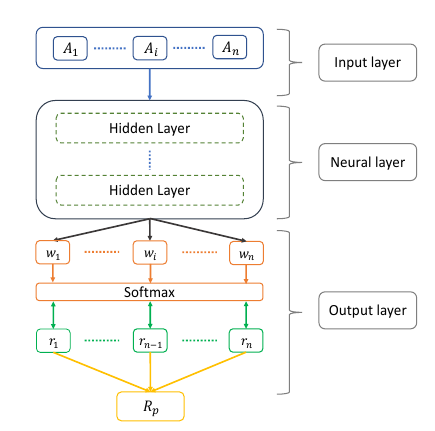
\includegraphics{images/Figure 1.png}
    \caption{Model architecture schematic}
    \label{fig:mesh1}
\end{figure}
\begin{description}
\item [Initial layer]  Each asset is designated as $A_{i}$, and a total of $n$ assets make up the portfolio. Concatenating data from all assets creates a single input. The historical prices and returns of one asset, for instance, might be the input features with a dimension of $(k, 2)$, where $k$ denotes the lookback window.
The input dimension would be $(k, 2\times n)$ if features were stacked across all assets. We may then feed this input into the network and anticipate the extraction of non-linear characteristics.
\item [The neural layer] A network may be created by stacking a number of hidden layers together; however, in fact, this step involves a lot of trials since there are several methods to combine hidden layers and the performance often relies on the architecture's design. Long Short-Term Memory (LSTM), Convolutional Neural Networks (CNN), and Fully Connected Neural Networks (FCN) have all been put to the test \cite{Hochreiter1997}. According to several studies \cite{Tsantekidis2017}, \cite{Lim2020} , LSTMs provide the greatest overall performance for modelling daily financial data.\\\\
We see that the extreme overfitting issue with FCN is a concern. There are too many parameters as a consequence of it giving parameters to each input characteristic. The LSTM uses a cell structure with gate mechanisms to summarise and filter data from its extensive history, resulting in fewer trainable parameters and higher generalisation outcomes. As a result, oversmooth solutions are produced when CNNs with significant smoothing (typical of large convolutional filters) are used. We see that the convolution procedures and the parameter sharing architecture cause CNNs to overfilter the inputs. We do, however, point out that CNNs seem to be top-notch contenders for modelling high-frequency financial data, such as limit order books.
\item [Outer layer] We use the \emph{softmax} activation function for the output layer to create a long-only portfolio, which by default applies restrictions to maintain portfolio weights in the positive and summing to one. We may multiply these portfolio weights by the related assets' returns $(r_{1}, r_{2},\cdots, r_{n}$) to get the realised portfolio returns since the number of output nodes ($w_{1}, w_{2},\cdots, w_{n})$ equals the number of assets in our portfolio $(R_{p} )$. After obtaining the realised returns, we may compute the Sharpe ratio's gradients with respect to the model's parameters and apply gradient ascent to update the parameters.
\end{description}